%Mid-Year Cadidature Review Report 
%Updated on 23/08/2012 at 15.30

\documentclass{article}  
\usepackage{a4wide}
\usepackage{amsmath,amssymb}
\usepackage{graphicx}
\usepackage{url}
\usepackage{tabulary}
\usepackage[sort]{cite}
%\usepackage[sort,nocompress]{cite}
\usepackage{multirow}
\usepackage{booktabs}
\usepackage{placeins}
\usepackage{caption}
\usepackage{subcaption}
\usepackage{epstopdf}
\usepackage{enumerate}
\usepackage{pdfpages}
\newcommand{\hilight}[1]{\colorbox{yellow}{#1}}

%\title{\Huge bfseries{Towards a green optical Internet 
%jnvsjkvnsfjkvnfkjsv 
%dfdfd
%}} 
%\author{\textsf{M. Nishan Dharmaweera}} 

%\year{April, 2004} 
%\department{\emph{Department of Electrical and Computer Systems Engineering}}
%\title{Towards a Green Optical Internet}
%\author{Nishan Dharmaweera \and Rajendran Parthiban \and Y. Ahmet \c{S}ekercio\u{g}lu}
\begin{document}

\begin{titlepage}
\begin{center}
{\huge \bfseries Energy harvesting using aeroelastic galloping}\\[2.5cm]
{\LARGE \bfseries H.G.K.G Jayatunga}\\[2.5cm]
\textsc{\Large Supervisors:\\[0.5cm] Dr. Tan Boon Thong \\[0.4cm] Dr. Justin Leontini \\[0.5cm] Dr Huang Yew Mun}\\[6.5cm]
\textsc{\Large Ph.D. Mid-Candidature Review Report}\\

\vfill
\textsc{\Large $27^{\text{th}}$ September 2013}
\end{center}
\end{titlepage}
%\titlepage
%\maketitle
\tableofcontents

\section{Introduction}
The search for alternative energy sources which could be categorised under the ”green” label has become important area of research in the modern word. Solar, wind power and wave power are some of the examples of these sources. Recently,a new branch of research has been developing to extract energy from flow induced vibrations. It has been hypothesized that this technique may work efficiently in areas where regular turbines cannot.
A simple structure that is susceptible to flow-induced vibrations that are suitable for energy extraction are slender structures,such as cylinders, elastically mounted perpendicular to a fluid stream. With regards to a slender body two common types of   flow induced vibrations are Vortex Induced Vibrations (VIV) and aeroelastic galloping. Significant research has been carried out by Bernitsas and his team on extracting useful energy from VIV. Some of their significant work includes investigating the influence  of physical parameters such as mass ratio (the ratio of the mass of the cylinder and the displaced fluid), Reynolds number, mechanical properties(\cite{Raghavan2010a} ,\cite{Lee2011b}) and location (effect of the bottom boundary) (\cite{Raghavan2009}). However,the possibility of extracting energy using aeroelastic galloping has not been thoroughly investigated. Some theoretical work was carried out by (\cite{Barrero-Gil2010a}). Utilizing galloping may be a more viable method to harness energy from flow induced vibrations as it is not bounded by a "lock-in" range of reduced velocities(ratio between the freestream velocity and the product of the natural frequency of the system and the characteristic length).Therefore it is preferable to investigate further the possibility of harnessing energy from flow induced vibrations using aeroelastic galloping. 

\section{Research focus}
 This research contributes to the existing knowledge on energy extraction from flow induced vibrations. The main focus is investigating methods to optimise the energy transfer from fluid-to-body when galloping by using theoretical methods (i.e Quasi-steady state theory and DNS simulations). Therefore the project was separated into two main phases.
 
\begin{enumerate}[]
\item Phase 1: Optimise the mechanical characteristics of the system.
\item Phase 2: Optimise the fluid dynamics portion of the system 
\end{enumerate}

\section{Research objectives}




\section{Research progress}

\subsection{Phase-1}

Phase 1 has been completed which is investigating the behaviour of the mechanical characteristics of the system. The following conclusions were made. Further information could be found in \hilight{Appendix}

\begin{itemize}
\item   the system is not frequency dependent, but more dependent on the velocity amplitude.
\item The main tuning parameter on the mechanical system to obtain an optimum power output is the damping factor.
\end{itemize}

\subsection{Phase-2}

As previously mentioned the fluid dynamics portion of the system is studied in phase-2.

\subsubsection{Creation of the negative lift}

In order to carry out an optimisation study on the fluid dynamics portion of the system, it is essential to study underlying fluid mechanics for galloping. It has been already established by \cite{Parkinson1964} that the instantaneous lift is the input of the system. Therefore it is essential to have an understanding on how exactly this lift occur. According to \cite{Parkinson1989},\hilight{Luo 94} the lift force is crated by the secondary flow of the two shear layers of either side of the body which creates an unbalanced pressure distribution on the afterbody. If a square cross section is taken as an example, when the body have a transverse $\dot{y}$, the relative velocity causes an instantaneous angle of attack which makes one shear layer lies closer to the body than the other. Therefore the shear layer near the body creates a pressure imbalance by creating a higher suction on the wall of the body on the adjacent side than the suction caused by the shear layer on the opposite side on its adjacent side of the body. The lift force become its maximum when the shear layer closer to the body re attaches at the trailing edge. As the angle of attack is further increased, the separated shear layer in the opposite side of the body (which was initially away from the body) shrinks therefore the pressure difference decreases which results a decrease in the lift force. This explanation was validated by \cite{Luo1994} by conducting flow visualisation experimentally.

Therefore two parameters could be identified which governs the lift 

\begin{itemize}
\item{ The characteristics of the afterbody}
\item{Shear layer separation}
\end{itemize}
 
\cite{Luo1994} have done some interesting studies on the lift characteristics on trapezoidal bodies. Which essentially the top and bottom sides of a square were tapered away systematically until it becomes triangle which is depicted in \hilight{Figure}.
\begin{figure}
  \centering
\fbox{
  \setlength{\unitlength}{\textwidth}
  \begin{picture}(0.6,0.5)

  
    % % %90
      \put(-0.1,0){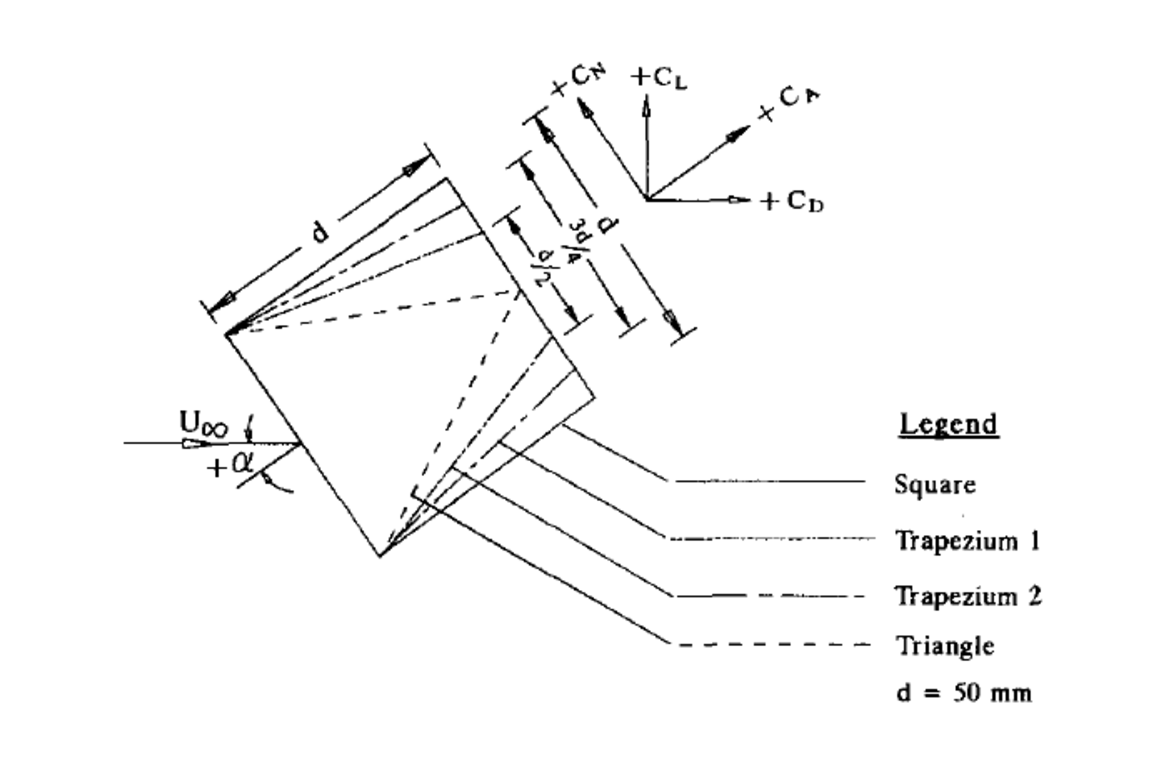
\includegraphics[width=0.75\unitlength]{./fnp/sketch-1.eps}}
     
% 	\put(0.02,0.93){ \large $C_y$} 	
%% 	\put(0.56,1.02){ $\theta$}
% 	
%        \put(0.25,0.8){ $\theta$} 	
%        \put(0.75,0.8){ $\theta$}
%        
%        \put(0.105,1.01){(a)}
%        \put(0.565,1.01){(b)}
     \end{picture}

 }
 \caption{Cross sectional shape considerd in in \cite{Luo2003}}
    \label{fig:lift_curves}
\end{figure}
. According to the data presented \cite{Luo1994} the highest lift is produced by the triangle. However, the maximum lift occur at a very large angle of attack ($\theta\approx 34^0 $) compared to a square cross section ($\theta\approx 12^0 $).

According to the literature survey carried out so far, investigations have been carried out only for 

   



 






 

%\begin{figure}[h]
%\centering
%\includegraphics[width=\textwidth]{./Gantt}
%\caption{Revised Gantt Chart}
%\label{fig:Gantt}
%\end{figure}


%\section{Difficulties and challenges} 
%%
%%\begin{enumerate}
%%      
%%\end{enumerate}
%\bibliographystyle{elsarticle-harv}
%\bibliography{../bibtex/MCR}
%\appendix
%%\begin{center}
%%\section*{\LARGE Appendix 1}
%%\addcontentsline{toc}{section}{Appendix 1} 
%%\end{center}
%Proposed table of contents of the final PhD thesis:
%\begin{enumerate}
%\item Introduction
%\begin{enumerate}[i]
%\item Looking forward
%\item Scope of the thesis
%\item Organization of the thesis
%\item Objectives
%\item Contributions
%\item Publications 
%\end{enumerate}
%\item Power consumption in optical core network
%\begin{enumerate}[i]
%\item Introduction
%\item Core network architecture
%\item Core node architecture 
%\item Power consumption values
%\item Node-based approaches
%\item Traffic engineering-based approaches
%\item Network engineering-based approaches
%\end{enumerate}
%\item Node-based energy efficiency
%\begin{enumerate}[i]
%\item Introduction
%\item General network model
%\item Problem definition
%\item Cost model
%\item Energy and cost efficient algorithm
%\item Framework for energy efficient OBS network
%\item Summary
%\end{enumerate}
%\item Traffic engineering-based energy efficiency
%\begin{enumerate}[i]
%\item Introduction
%\item Grooming based network model
%\item Problem definition
%\item Sparse grooming 
%\item Waveband grooming 
%\item Summary
%\end{enumerate}
%\item Network engineering-based energy efficiency \begin{enumerate}[i]
%\item Introduction
%\item MLR based network model
%\item Problem definition
%\item MLR based WBS network
%\item Sleep mode enabled core network
%\item Summary
%\end{enumerate}
%\item Conclusion
%\begin{enumerate}[i]
%\item Introduction
%\item Summary of the work
%\item Future directions
%\end{enumerate}
%\end{enumerate}
%Each sub-section mentioned above could be further divided into sections, if necessary. For example, 3(v) could be divided as 3(v)(a) "ILP formulation", 3(v)(b) "Heuristic algorithm" and 3(v)(c) "Evaluation"
%\newpage
%\centering
%\vspace*{2.5in}

\end{document}